\section*{Zadanie 11.}
\begin{task}

Dane są rezonatory o ściankach idealnie przewodzących: 
\begin{enumerate}[a)]
\item Prostopadłościenny o wymiarach (podane kolejno w kierunki osi x,y i z) a = 3cm, b = 4cm i c = 10cm;
\item Cylindryczny o średnicy d = 10cm i wysokości h = 2cm.
\end{enumerate}
W każdym przypadku nazwać dwa rodzaje rezonansowe o najniższych częstosliwościach, obliczyć ich częstotliwości drgań własnych oraz naszkicować rozkłady pola elektrycznego w każdym z nich.\\

\end{task}


\begin{solution}
\begin{enumerate}[a)]

\item $\lambda_{rez} = \frac{2}{\sqrt{(\frac{m}{a})^2+(\frac{n}{b})^2+(\frac{p}{c})^2}} \\
f_{rez} = \frac{c}{\lambda_{rez}} \qquad$
$f_{rez} = \frac {c \cdot \sqrt{(\frac{m}{a})^2+(\frac{n}{b})^2+(\frac{p}{c})^2}}{2}$\\

Obliczenia dla rodzaju H (TE): \\
$f_{011} = \frac{3 \cdot 10^8}{2} \cdot \sqrt{(\frac{0}{0,03})^2+(\frac{1}{0,04})^2+(\frac{1}{0,1})^2} = 4038873605,351 Hz = \underline{4,04 GHz} $\\
$f_{101} = \frac{3 \cdot 10^8}{2} \cdot \sqrt{(\frac{1}{0,03})^2+(\frac{0}{0,04})^2+(\frac{1}{0,1})^2} = 5220153254,455 Hz = 5,22 GHz $\\
$f_{111} = \frac{3 \cdot 10^8}{2} \cdot \sqrt{(\frac{1}{0,03})^2+(\frac{1}{0,04})^2+(\frac{1}{0,1})^2} = 6427480066,091 Hz = 6,43 GHz$\\
\begin{center}
    $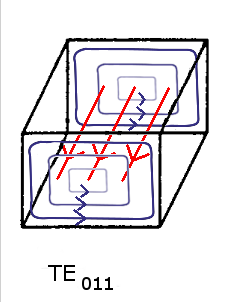
\includegraphics[scale=1]{11_1}$\\
\end{center}

Obliczenia dla rodzaju E (TM): \\

$f_{211} = \frac{3 \cdot 10^8}{2} \cdot \sqrt{(\frac{2}{0,03})^2+(\frac{1}{0,04})^2+(\frac{1}{0,1})^2} = 10784827305,062 Hz = 10,78 GHz $\\
$f_{111} = \frac{3 \cdot 10^8}{2} \cdot \sqrt{(\frac{1}{0,03})^2+(\frac{1}{0,04})^2+(\frac{1}{0,1})^2} = 6427480066,091 Hz =  \underline{6,43 Ghz}$\\
$f_{112} = \frac{3 \cdot 10^8}{2} \cdot \sqrt{(\frac{1}{0,03})^2+(\frac{1}{0,04})^2+(\frac{2}{0,1})^2} = 6932712311,931 Hz = 6,93 GHz $\\
$f_{121} = \frac{3 \cdot 10^8}{2} \cdot \sqrt{(\frac{1}{0,03})^2+(\frac{2}{0,04})^2+(\frac{1}{0,1})^2} = 9137833441,249 Hz = 9,15 GHz$\\
\begin{center}
    $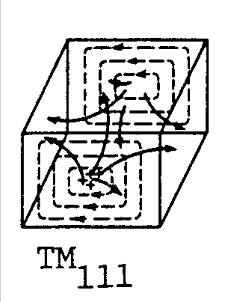
\includegraphics[scale=1]{11_2}$\\
\end{center}

\item W rezonatorze cylindrycznym warunki brzegowe uniemożliwiają utworzenie się rodzaju $H_{mn0} (TE_{mn0})$\\. \\
Pulsacja drgań własnych dla rodzaju H (TE): \\
 $\omega_v = \frac{1}{\sqrt{\mu \varepsilon}} \cdot \sqrt{(\frac{ \chi'_{mn} }{d})^2+(\frac{ \pi }{h})^2} $\\
$\omega_v = 2 \cdot \pi \cdot f_v$\\
$f_v = \frac{\omega_v}{2\cdot \pi} $\\
$f_v = \frac{1}{2\pi\sqrt{\mu \varepsilon}}\sqrt{(\frac{ \chi'_{mn} }{d})^2+(\frac{ \pi }{h})^2} $\\
$\sqrt{\mu_0 \varepsilon_0}=3,33 \cdot 10^{-9}$ \\

    \begin{center}
        $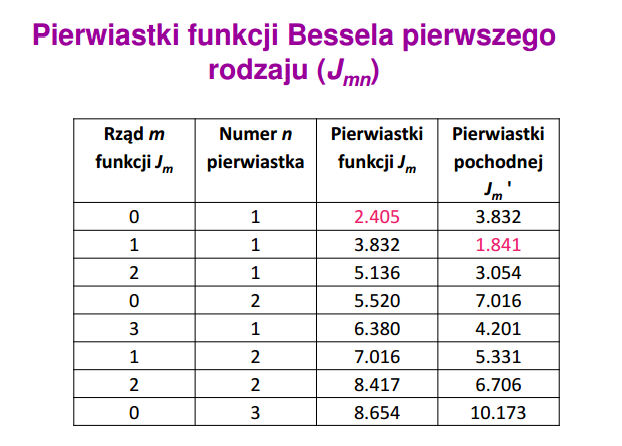
\includegraphics[scale=1]{11_bessel}$\\
    \end{center}

$f_{01p} = \frac{1}{2\pi \cdot 3,33 \cdot 10^{-9}}\sqrt{(\frac{ \chi'_{01} }{0,1})^2+(\frac{ \pi }{0,02})^2} = 7,72 GHz$\\
$f_{11p} = \frac{1}{2\pi \cdot 3,33 \cdot 10^{-9}}\sqrt{(\frac{ \chi'_{11} }{0,1})^2+(\frac{ \pi }{0,02})^2} = \underline{7,55 GHz}$\\
$f_{21p} = \frac{1}{2\pi \cdot 3,33 \cdot 10^{-9}}\sqrt{(\frac{ \chi'_{21} }{0,1})^2+(\frac{ \pi }{0,02})^2} = 7,64 GHz$\\
$f_{02p} = \frac{1}{2\pi \cdot 3,33 \cdot 10^{-9}}\sqrt{(\frac{ \chi'_{02} }{0,1})^2+(\frac{ \pi }{0,02})^2} = 8,21 GHz$\\
$f_{31p} = \frac{1}{2\pi \cdot 3,33 \cdot 10^{-9}}\sqrt{(\frac{ \chi'_{31} }{0,1})^2+(\frac{ \pi }{0,02})^2} = 7,76 GHz$\\
$f_{12p} = \frac{1}{2\pi \cdot 3,33 \cdot 10^{-9}}\sqrt{(\frac{ \chi'_{12} }{0,1})^2+(\frac{ \pi }{0,02})^2} = 7,92 GHz$\\
$f_{22p} = \frac{1}{2\pi \cdot 3,33 \cdot 10^{-9}}\sqrt{(\frac{ \chi'_{22} }{0,1})^2+(\frac{ \pi }{0,02})^2} = 8,16 GHz$\\
$f_{03p} = \frac{1}{2\pi \cdot 3,33 \cdot 10^{-9}}\sqrt{(\frac{ \chi'_{03} }{0,1})^2+(\frac{ \pi }{0,02})^2} = 8,93 GHz$\\

    \begin{center}
        $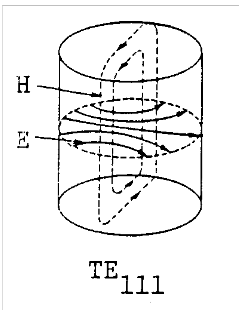
\includegraphics[scale=1]{11_3}$\\
    \end{center}

Dla rodzaju E w falowodzie $\beta_g = \frac{\chi_mn}{d}$ więc pulsacja drgań własnych pola rodzaju E wynosi \\
$f = \frac{1}{2\pi\sqrt{\mu \varepsilon}} \cdot \frac{\chi_{mn}}{d}$\\
$\sqrt{\mu_0 \varepsilon_0}=3,33 \cdot 10^{-9}$ \\
\\
$f_{01p} = \frac{1}{2\pi\sqrt{\mu \varepsilon}} \cdot \frac{\chi_{01}}{0,1} = \underline{1,15 GHz}$\\
$f_{11p} = \frac{1}{2\pi\sqrt{\mu \varepsilon}} \cdot \frac{\chi_{11}}{0,1} = 1,83 GHz$\\
$f_{21p} = \frac{1}{2\pi\sqrt{\mu \varepsilon}} \cdot \frac{\chi_{21}}{0,1} = 2,45 GHz$\\
$f_{02p} = \frac{1}{2\pi\sqrt{\mu \varepsilon}} \cdot \frac{\chi_{02}}{0,1} = 2,64 GHz$\\
$f_{31p} = \frac{1}{2\pi\sqrt{\mu \varepsilon}} \cdot \frac{\chi_{31}}{0,1} = 3,05 GHz$\\
$f_{12p} = \frac{1}{2\pi\sqrt{\mu \varepsilon}} \cdot \frac{\chi_{12}}{0,1} = 3,35 GHz$\\
$f_{22p} = \frac{1}{2\pi\sqrt{\mu \varepsilon}} \cdot \frac{\chi_{22}}{0,1} = 4,02 GHz$\\
$f_{03p} = \frac{1}{2\pi\sqrt{\mu \varepsilon}} \cdot \frac{\chi_{03}}{0,1} = 4,13 GHz$\\

    \begin{center}
        $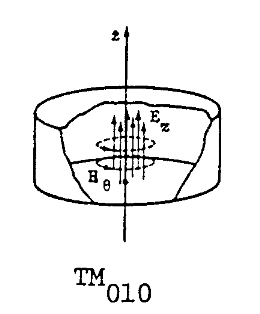
\includegraphics[scale=1]{11_4}$\\
    \end{center}
    \end{enumerate}
\end{solution}